%\begin{frame}{EPAM}
%  \begin{center}
%    
\includegraphics[height=3.3cm]{epam}
%  \end{center}
%\end{frame}

\begin{frame}{}
	\begin{columns}
		\column{0.7\textwidth}
		\Huge
		\center{Developers!\\Developers!\\Developers!\\}
		\column{0.3\textwidth}
		\center
\includegraphics[height=4cm]{steve_ballmer}
	\end{columns}
\end{frame}


\begin{frame}
	\frametitle{Курсы Linux от Epam}

	\begin{block}{Цели}
		\begin{itemize}
			\item Увеличение популярности GNU/Linux среди программистов
			\item Воспитание потенциальных сотрудников
		\end{itemize}
	\end{block}

	\pause

	\begin{block}{Целевая аудитория}
		\begin{itemize}
			\item Студенты технических специальностей
			\item Программисты, желающие освоить работу в ОС Linux
		\end{itemize}
	\end{block}

	\begin{block}{Требования к кандидатам}
		\begin{itemize}
			\item Уметь программировать, под любую платформу.
		\end{itemize}
	\end{block}
\end{frame}

\begin{frame}
	\frametitle{Программа}

	\begin{block}{Командная строка -- важнейший инструмент понимания процесса разработки}
		\begin{itemize}
			\item Представление об архитектуре GNU/Linux дистрибутива
			\item Введение в shell-программирование
			\item Классические средства разработки, отладки и оптимизации
		\end{itemize}
	\end{block}
\end{frame}

\begin{frame}
	\frametitle{Формат проведения занятий}

	\begin{block}{Принципы}
		\begin{itemize}
			\item Лекторы? Учителя? {\bf NO WAY!!!} \newline 
				Разработчики для разработчиков! 
			\item Небольшая группа изучающих
			\item Балланс между теорией и практикой
		\end{itemize}
	\end{block}

\end{frame}

\begin{frame}
  \frametitle{Первый набор}
  \begin{columns}
    \column{0.5\textwidth}
	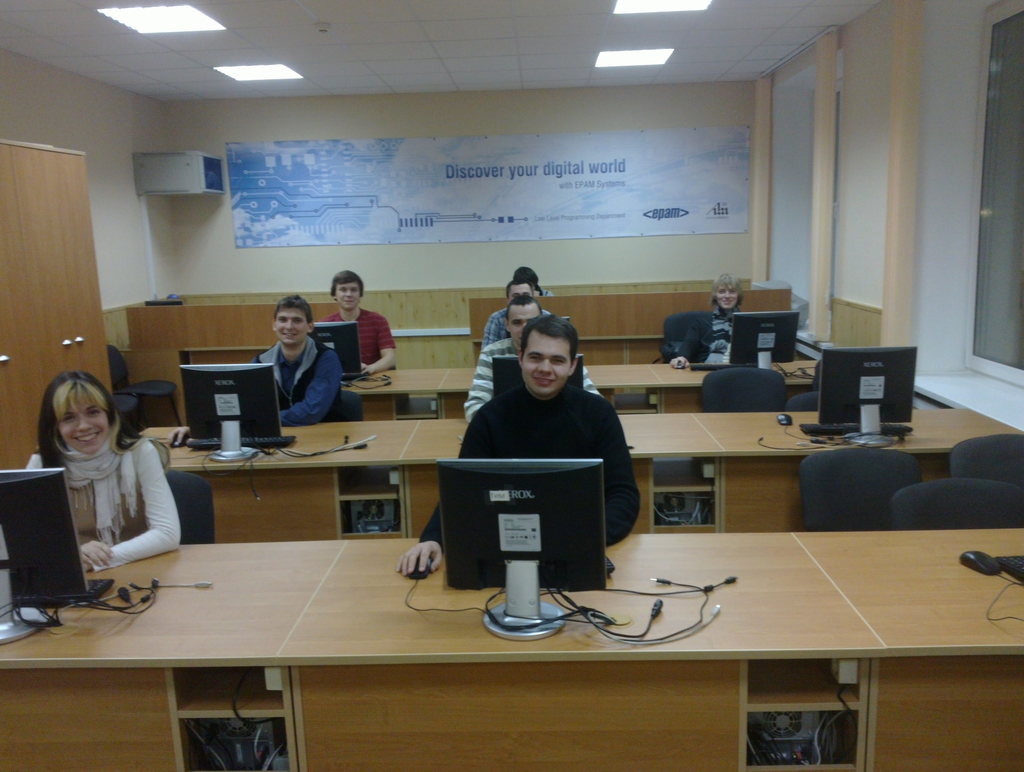
\includegraphics[width=\textwidth]{epam-evm_lab512}

    \column{0.5\textwidth}
	\begin{block}{Немного статистики}
		\begin{itemize}
			\item Подано заявок: {\bf 39} человек
			\item После первоначального отбора: {\bf 16} человек
				\begin{itemize}
					\item из них {\bf 4} -- сотрудники Epam
				\end{itemize}
            \item Получили сертификаты человек
            \item Планировали 48 часов
            \pause
            \item Получилось 66 часов
		\end{itemize}
	\end{block}
  \end{columns}

    
\end{frame}

\begin{frame}
  \frametitle{Успех!}
  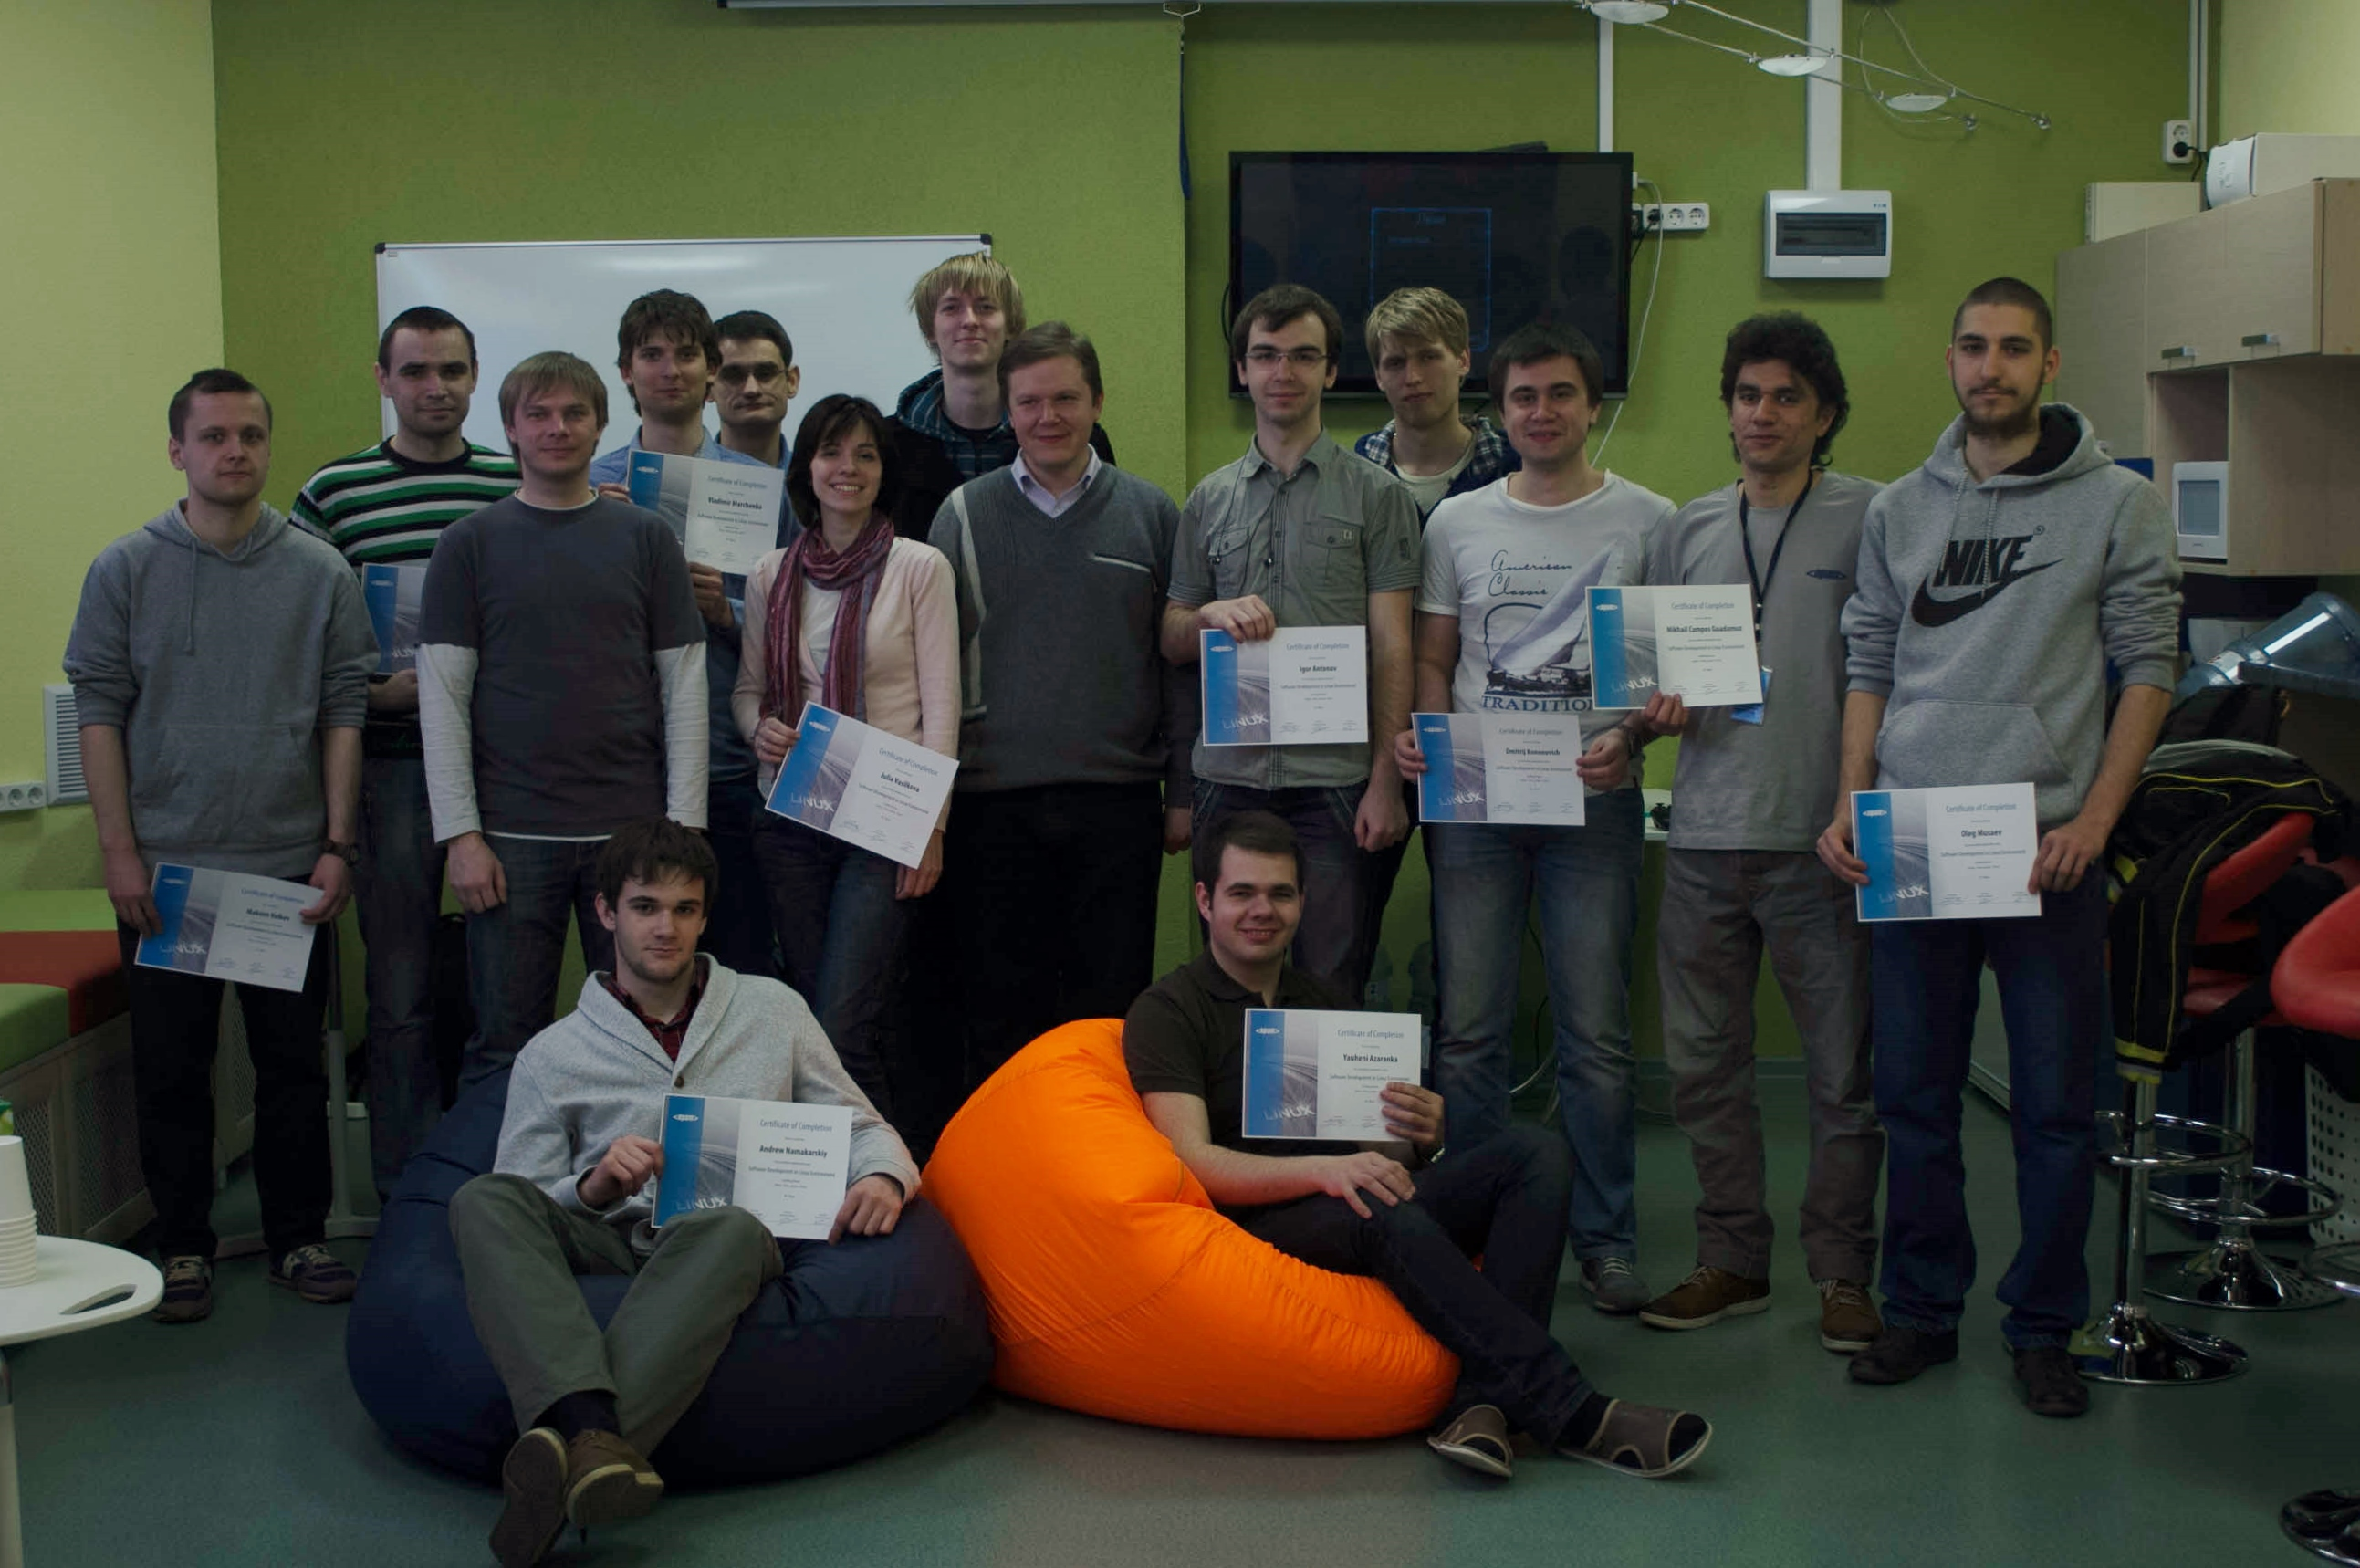
\includegraphics[width=\textwidth]{linux_courses_certificates1.jpg}
\end{frame}

\begin{frame}
  \frametitle{Работа над ошибками}
  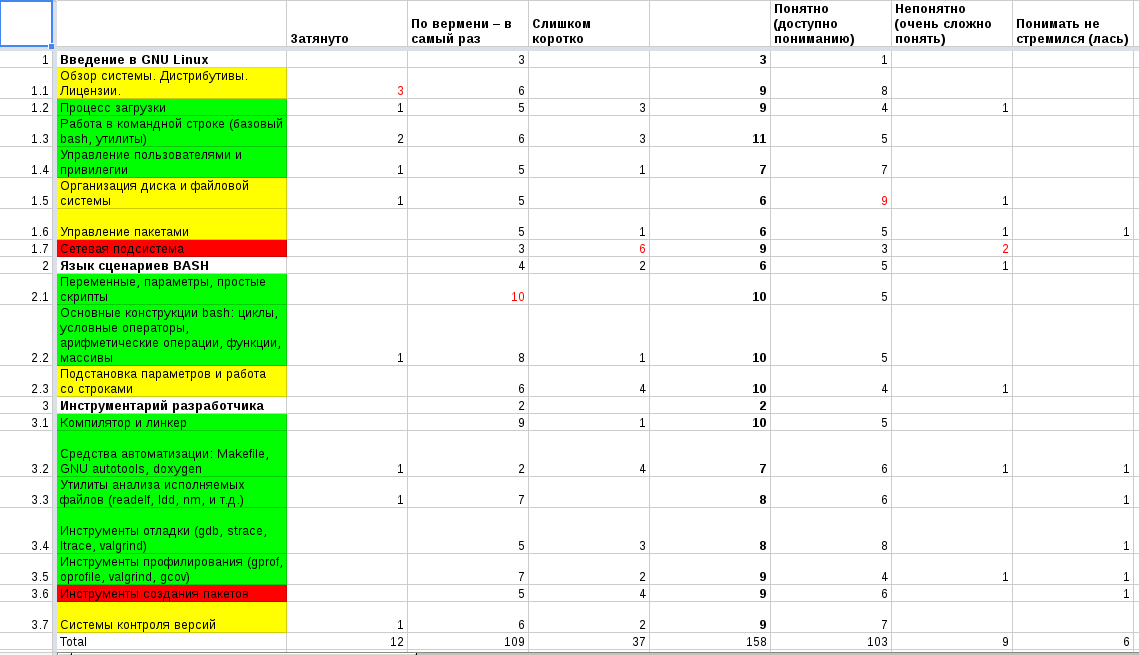
\includegraphics[width=\textwidth]{anketa.png}
\end{frame}

\begin{frame}
\frametitle{Второй набор}
  \begin{itemize}
    \item Пересмотрены некоторые разделы (networking, лицензии)
    \item Два новых лектора
    \item Добавлены новые разделы
      \begin{itemize}
        \item Python
        \item C
      \end{itemize}
  \end{itemize}
 \begin{block}{Статистика}
    \begin{itemize}
      \item Подано заявок: ?
      \item Предварительно отобрано: 15 человек
      \item На занятиях: 11 человек + сотрудники EPAM (6-8 посещение свободное)
      \item Один человек нашел работу в процессе
    \end{itemize}
  \end{block}
\end{frame}

\begin{frame}
  \frametitle{Оргвыводы по второму набору}
  \begin{itemize}
    \item
  \end{itemize}
\end{frame}
